%%% Local Variables:
%%% mode: latex
%%% TeX-master: t
%%% End:
% --------------------------------------------------------------
% This is all preamble stuff that you don't have to worry about.
% Head down to where it says "Start here"
% --------------------------------------------------------------

\documentclass[12pt]{article}

\usepackage[margin=1in]{geometry}
\usepackage{amsmath,amsthm,amssymb}
\usepackage{graphicx}

\newcommand{\N}{\mathbb{N}}
\newcommand{\Z}{\mathbb{Z}}

\newenvironment{theorem}[2][Theorem]{\begin{trivlist}
\item[\hskip \labelsep {\bfseries #1}\hskip \labelsep {\bfseries #2.}]}{\end{trivlist}}
\newenvironment{lemma}[2][Lemma]{\begin{trivlist}
\item[\hskip \labelsep {\bfseries #1}\hskip \labelsep {\bfseries #2.}]}{\end{trivlist}}
\newenvironment{exercise}[2][Exercise]{\begin{trivlist}
\item[\hskip \labelsep {\bfseries #1}\hskip \labelsep {\bfseries #2.}]}{\end{trivlist}}
\newenvironment{reflection}[2][Reflection]{\begin{trivlist}
\item[\hskip \labelsep {\bfseries #1}\hskip \labelsep {\bfseries #2.}]}{\end{trivlist}}
\newenvironment{proposition}[2][Proposition]{\begin{trivlist}
\item[\hskip \labelsep {\bfseries #1}\hskip \labelsep {\bfseries #2.}]}{\end{trivlist}}
\newenvironment{corollary}[2][Corollary]{\begin{trivlist}
\item[\hskip \labelsep {\bfseries #1}\hskip \labelsep {\bfseries #2.}]}{\end{trivlist}}

\begin{document}

% --------------------------------------------------------------
%                         Start here
% --------------------------------------------------------------

%\renewcommand{\qedsymbol}{\filledbox}

\title{CS5214 Design of Optimizing Compilers }%replace X with the appropriate number
\author{Professor Weng-Fai Wong\\ %replace with your name
Assignment Two} %if necessary, replace with your course title

\maketitle

\abstract{This is the answer presented by Pan An. My student number is
  A0134556A. After tryin all the cool tools in Python, GNUPlot, and
  some books and papers, I finally figured out that this assignment is
not about programming. Alright so I'm just gonna present some results
that are partially calculated with my hand. Some of the math greatly
damaged my brain(kidding). Also I wanted to put a lot of references
but it seems that time is not enough for that. The folder contains
some of the rough calculation results performed by Python and some
other tools.}
% --------------------------------------------------------------
%     You don't have to mess with anything below this line.
% --------------------------------------------------------------
\section{The Lengauer‐Tarjan algorithm}

For the first question I simply assumn that in this diagram it does
not have very terrible effect by counting the {\bf start} and {\bf
  stop} nodes into the algorithm.

\subsection{Depth First Search}
I simply used {\bf networkx} in Python to do some of the graph
operation for me. The depth first search tree is stored in a picture
in {\bf img folder}.

After performing DFS on the tree, the DFT numbering is listed below in
the form of ($n_{DFT}$, Node). Node with number 0 and 100 are the
start and stop node.

\begin{verbatim}
(1, 0)
(2, 1)
(3, 2)
(4, 8)
(5, 31)
(6, 4)
(7, 5)
(8, 6)
(9, 7)
(10, 9)
(11, 10)
(12, 11)
(13, 12)
(14, 13)
(15, 14)
(16, 15)
(17, 16)
(18, 33)
(19, 18)
(20, 34)
(21, 21)
(22, 100)
(23, 3)
(24, 17)
(25, 19)
\end{verbatim}
Noticing that there could be multiple answers to DFS tree numbering, I
am using this one as the answer for the next couple questions.

\subsection{Dominators}
Most of the time semi-dominators of nodes in a graph is the immediate
dominator. The following picture shows the semi-dominator of the given
diagram:

\begin{figure}
\centering
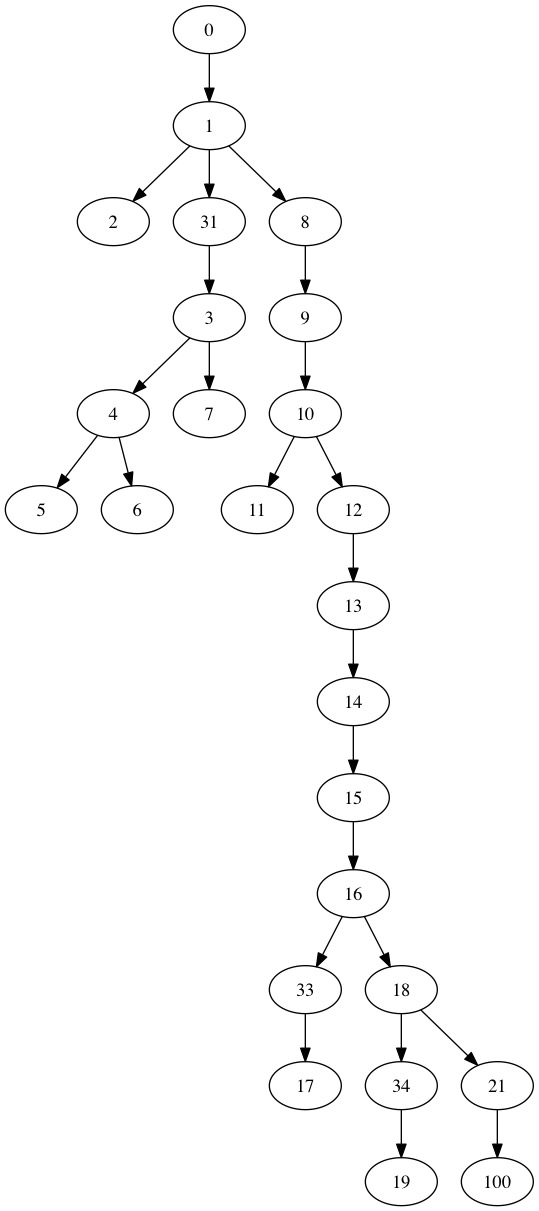
\includegraphics[scale=0.35]{imdom.jpg}
\caption{Semi Dominator Graph}
\end{figure}

\subsection{Control Dependency}
Actually I am a little  skeptical about this one since I actually read
another source that it does not have to be strict dominance in the
definition of control dependence.
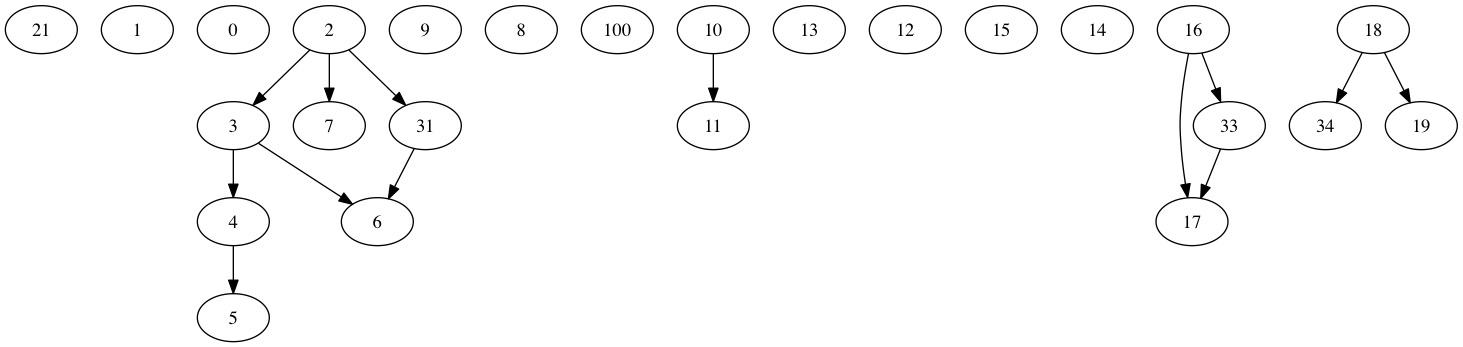
\includegraphics[scale=0.3]{cdg.jpg}

\subsection{Strongly Connected Componants}
A directed graph is called strongly connected if there is a path in
each direction between each pair of vertices of the graph.

Strongly connected graphs are(all edges amongs these nodes included):

\begin{itemize}
\item Nodes with self loop: 9, 13, 15, 19
\item Graph composed with node 16 and 33
\item Graph composed with node 3, 4, 6, 7
\item Graph composed with node 3, 4, 6, 7, 5
\item Graph composed with node 9, 10, 11
\end{itemize}


\subsection{Question 7}

Dominant frontiers of the three nodes are:
\begin{itemize}
\item 31: [8]
\item 11: [9, 12]
\item 33: [16, 18]
\end{itemize}

\noindent
Block 8, 9, 12, 16, 18 should be inserted with $\phi$ function.

\section{ Dataflow analysis}
To be honest, I lost it when it comes to this part in the class so I
Wikipediaed a little. Also I read the slides but the slides seem not
so fullfilled in this part(no offence).  So here I will just use the
expression in terms of data flow equations.

The problem is a typical backward data flow analysis problem. Let
$def[n]$ be the set of variables that are used in node n before any
assignment. The function $use[n]$ with lower case letters does the
exact same thing as $USE[n]$. Let $succ[n]$ be the set of successor nodes
after node n successfully excutes. Dataflow equations can be expressed as the following:
\begin{itemize}
\item $live_{in}[n] = def[n] \cup (live_{out}[n] - use[n])$
\item$live_{out}[final] = \Phi$
\item$live_{out}[n] =\bigcup_{p\in succ[n]}live_{in}[p] $
\end{itemize}


The algorithm for solving data flow equation is presented below:


{\bf for each} node n in CFG:\\
\indent
~~~~$live_{in}[n] = \Phi, live_{out}[n] = \Phi$\\
\indent
{\bf repeat}\\
\indent
~~~~{\bf for each} node n in CFG:\\
\indent
~~~~~~~~ $ live'_{in}[n] = live_{in}[n]$\\
\indent
~~~~~~~~ $ live'_{out}[n] = live_{out}[n]$\\
\indent
~~~~~~~~ $ live_{in}[n] = use[n] \cup (live_{out}[n] - def[n])$\\
\indent
~~~~~~~~ $live_{out}[n] =\bigcup_{p\in succ[n]}live_{in}[p] $\\
\indent
{\bf until }$live'_{in}[n] = live_{in}[n]  and live'_{out}[n] =
  live_{out}[n] for all n $

%The algorithm can be considered finding all the nodes that will never
%go through those nodes with
% with the $USE(n)>0$ it reaches {\bf stop}. Also the node should be the 'first
%one'.



Consider the following graph:

\begin{figure}
\centering
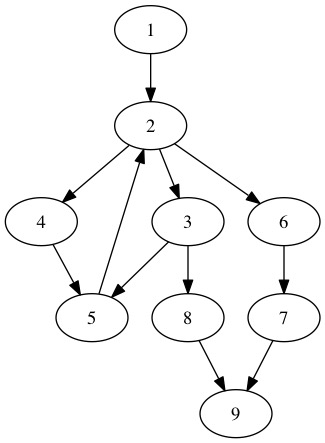
\includegraphics[scale=0.5]{example.jpg}
\end{figure}
Assuming  that in the graph node {\bf 3 and 5} are with a postive
$USE(n)$ value(variable is used) and the variable is {\bf defined} in
block 1. The algorithm will first traverse
the graph and find the variable usage, and after this process:
$$S_{u} = \{3, 5\}$$


Here I assumn there are couple things happening:
\begin{enumerate}
\item In node 1:
  \begin{itemize}
  \item a = 2;
\item b = 1;
\item c = 1;
  \end{itemize}
\item Node 2: a = 1, 2, 3, means switch to 4, 3, 6;
\item Node 5:
  \begin{itemize}
  \item c = a - b;
    \item d = 2;
  \end{itemize}
\item Node 3:
  \begin{itemize}
    \item d = c + 1;
    \item if a $>$ d then go to 8, else go to 5;
  \end{itemize}
\item Nothing concerns a, b, c, d happens in other nodes;
\end{enumerate}

The program flow will be pretty simple:
$$1, in=\{\}, out=\{\} \rightarrow 2, in=a, out=\{\}\rightarrow 3,
in=acd, out=\{\}\rightarrow$$
$$
5, in=abcd, out=a\rightarrow 2 in=a, out=cd\rightarrow
3 in=acd, out=\{\}\rightarrow 8 in=\{\}till stop$$

\vspace{4mm}
So it actually only concerns nodes 1, 2, 3, 5, 8. And the last uses of
each variable can be tracked from the flow above.


\end{document}
